\chapter{Modeling doxycycline-induced mCherry expression systems, with feedback} % Main chapter title

\label{Part2_chapter} % For referencing the chapter elsewhere, use \ref{Chapter1} 



\section{Informations}

1. pCMV is a constitutive promoter.

2. Black triangle is a tetR-dimer binding site (tetO), there are two of them near TATA box

3. NLS is nuclear localization sequence, facilitate the translocation of tetR to nucleus.

4. In the absence of Doxcycline, tetR-dimer preferably binds to tetO, block the RNA polymerase.

5. In the presence of Doxcycline, tetR-dimer preferably disassociate from tetO, remove the interference to RNA polymerase.

\begin{figure}[th]
\centering
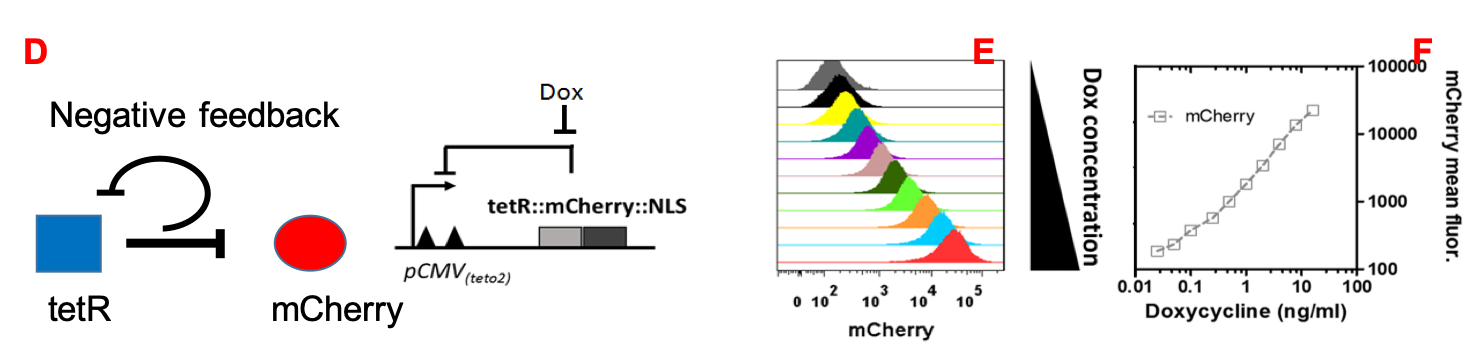
\includegraphics[width=1.0\linewidth]{Figures/part2.png}
\caption{Pictures of part 2}
\label{part_2_qestion_figure}
\end{figure}
%----------------------------------------------------------------------------------------
\section{Write step-by-step reactions}

\subsection{Symbols}

\begin{table}[H]
\caption{Modeling doxycycline-induced mCherry expression systems with feedback}
\label{tab:part2_symbols}
\centering
\begin{tabular}{l l}
\toprule

\tabhead{Symbol} & \tabhead{Definition} \\
\midrule
$D$ & The doxycycline molecular\\
$R$ & The tetR molecular\\
$R^{2}_{i}$ &   % ${\rm R^{2}_{i}}$ 改成正常体
The tetR-dimer molecular binds with \keyword{i} doxycycline molecular \\
$R^2$ & 
A mixture of $R^{2}_{0}$, $R^{2}_{1}$ and $R^{2}_{2}$\\
$O_{m}$ & 
The $tetO^{2}$ binding with m $R^{2}_{0}(m = 0, 1, 2)$\\
%\quad$O_{00}$ & 
%\quad Both two tetOs are free \\
%\quad$O_{10}$ & 
%\quad One tetO is free and another is occupied by $R^{2}_{1}$ \\
%\quad$O_{11}$ & 
%\quad Both two tetOs are occupied by $R^{2}_{1}$ \\
%\quad$O_{20}$ & 
%\quad One tetO is free and another is occupied by $R^{2}_{0}$ \\
%\quad$O_{21}$ & 
%\quad Two tetO are respectively occupied by a $R^{2}_{0}$ and a $R^{2}_{1}$\\
%\quad$O_{22}$ & 
%\quad Both two tetOs are occupied by $R^{2}_{0}$ \\
$O_{on}$ & 
The binding situation of $tetO^{2}$ that turn on the expression of GFP mRNA\\
$O_{sum}$ & 
Including $O_{0}, O_{1}, O_{2}$ \\
$C$ & 
mCherry protein \\
$P$ & 
RNA polymerase \\
$K_{1}$ & 
Reaction equilibrium constant of $R^{2}_{0}$ formation from $R$\\
$K_{2}$ & 
Reaction equilibrium constant of $R^{2}_{1}$ formation from $R^{2}_{0}$\\
$\sigma_{1}$ & 
$K_{3} = \sigma_{1} K_{2}$, \\ &so $\sigma_{1}$ represent binding strengths relative to the tetR-dimer-$tetO^{2}$ strength \\
$K_{3}$ & 
Reaction equilibrium constant of $R^{2}_{2}$ formation from $R^{2}_{1}$\\
$K_{4}$ & 
Reaction equilibrium constant of $O_{1}$ formation from $O_{0}$\\
$\sigma_{2}$ & 
$K_{5} = \sigma_{2} K_{4}$, \\ &so $\sigma_{2}$ represent binding strengths relative to the tetR-dimer-doxycycline strength \\
$K_{5}$ & 
Reaction equilibrium constant of $O_{2}$ formation from $O_{1}$\\
$k_{t}$ & 
Reaction constant of mCherry and tetR production\\
$k_{d-c}$ & 
Reaction constant of mCherry degradation\\
$k_{d-rd}$ & 
Reaction constant of tetR-dimer degradation\\
$P_{0}$ & 
I assume that the concentration of $P$ remains constant as $P_{0}$ during time\\
$n_c$ & 
The number of mCherry per mRNA transcript\\
$n_{rd}$ & 
The number of tetR-dimer per mRNA transcript\\
$r_c$ & 
The basal rate of production of mCherry\\
$r_{rd}$ & 
The basal rate of production of tetR-dimer\\
\bottomrule\\
\end{tabular}
\end{table}
\newpage


\subsection{Model}
The chemical reactions describing the network are naturally divided into two categories—fast and slow. The fast reactions have rate constants of order seconds and are therefore assumed to be in equilibrium with respect to the slow reactions, which are described by rates of order minutes.

Considering the reactions between tetR molecular, tetR-dimer molecular and doxycycline molecular, then we may write the equilibrium fast reactions :

\begin{equation} 
\begin{aligned} 
\centering
% \underset{A}{B}
% \overset{…}{…}
2R         &\underset{}{\overset{K_1}{\rightleftharpoons}} R^2_0 \\ 
R^2_0 + D  &\underset{}{\overset{K_2}{\rightleftharpoons}} R^2_1 \\ 
R^2_1 + D  &\underset{}{\overset{K_3}{\rightleftharpoons}} R^2_2 \\  
\end{aligned} 
\end{equation}

If we ignore the exsit of tetR molecular and assume all of them will take part in the formation of tetR-dimer molecular, in aother word, the $K_1$ is extrimly huge, the reactions become : 

\begin{equation} 
\begin{aligned} 
\centering
% \underset{A}{B}
% \overset{…}{…}
R^2_0 + D  &\underset{}{\overset{K_2}{\rightleftharpoons}} R^2_1 \\ 
R^2_1 + D  &\underset{}{\overset{K_3}{\rightleftharpoons}} R^2_2 \\  
\end{aligned} 
\end{equation}

Considering the reactions between tetR-dimer molecular and $tetO^{2}$, and it is assumed that the tetR-dimer binding with doxycycline molecular could not binding to $tetO^{2}$, then we may write the equilibrium fast reactions :

\begin{equation} 
\begin{aligned} 
\centering
% \underset{A}{B}
% \overset{…}{…}
O_0 + R^2_0  &\underset{}{\overset{K_4}{\rightleftharpoons}} O_1 \\ 
O_1 + R^2_0  &\underset{}{\overset{K_5}{\rightleftharpoons}} O_2 \\  
\end{aligned} 
\end{equation}

It is assumed that only $O_0$ can bind to $tetO^{2}$. \\
The slow reactions are transcription and degradation :

\begin{equation} 
\centering
\begin{aligned} 
% \underset{A}{B}
% \overset{…}{…}
\qquad \qquad \quad[O_{on}]    &= [O_0] \\
%\qquad \qquad \quad[O_{on}]    &= [O_0] + \frac{1}{2}[O_1] \\
\qquad \qquad \quad O_{on} + P &\underset{}{\overset{k_t}{\rightarrow}} 
O_{on} + P + n_cC + n_{rd}R^2\\ 
\qquad \qquad \quad C          &\underset{}{\overset{k_{d-c}}{\rightarrow}} 
\phi \\  
\qquad \qquad \quad R^2      &\underset{}{\overset{k_{d-rd}}{\rightarrow}} 
\phi \\  
\end{aligned} 
\end{equation}

The number of $tetO^{2}$ is depended by the number of plasmids in the cell. So the number of $tetO^{2}$ is a constant, which means $O_{sum}$ = $[O_0]+[O_1]+[O_2]$ does not change in a specific cell. Also, since the transcription reaction is slower than the reactions in Eq.2.1, the $R_0^2$ produced in transcription will partly become $R_1^2$ and $R_2^2$. So $R^2$ was used to donate this mixture of $R_0^2$, $R_1^2$ and $R_2^2$. $[R^2]$ = $[R_0^2]$ + $[R_1^2]$ + $[R_2^2]$

\subsection{Reactions}

\begin{equation*} 
\begin{aligned} 
\centering
% \underset{A}{B}
% \overset{…}{…}
R^2_0 + D    &\underset{}{\overset{K_2}{\rightleftharpoons}} R^2_1 \\ 
R^2_1 + D    &\underset{}{\overset{K_3}{\rightleftharpoons}} R^2_2 \\  
O_0 + R^2_0  &\underset{}{\overset{K_4}{\rightleftharpoons}} O_1 \\ 
O_1 + R^2_0  &\underset{}{\overset{K_5}{\rightleftharpoons}} O_2 \\ 
[O_{on}]     &= [O_0] \\
O_{on} + P   &\underset{}{\overset{k_t}{\rightarrow}} O_{on} + P + n_cC + n_{rd}R^2\\
C            &\underset{}{\overset{k_{d-c}}{\rightarrow}} \phi \\  
R^2        &\underset{}{\overset{k_{d-rd}}{\rightarrow}} \phi \\  
\end{aligned} 
\end{equation*}


%----------------------------------------------------------------------------------------

\section{Write ODE equations from reactions}

Form the reactions above, ODE equations could be written and we know that : 
\begin{equation} 
\begin{aligned} 
\centering
% \underset{A}{B}
% \overset{…}{…}
K_i &= \frac{k_i}{k_{-i}}(i = 2,3,4,5) \\
\frac{d[R_0^2]}{dt} &=  + k_{-2} [R^2_1] + k_{-4}[O_1] + k_{-5}[O_2] \\
				    &\qquad - (k_2[D]+k_4[O_0]+k_5[O_1]) [R_0^2] \\
\frac{d[R_1^2]}{dt} &= k_{-3}[R_2^2]-k_3[R^2_1][D]+k_2[R^2_0][D]-k_{-2}[R^2_1] \\
\frac{d[R_2^2]}{dt} &= k_{3}[R_2^1][D]- k_{-3}[R^2_2] \\
\frac{d[O_0]}{dt} &= k_{-4}[O_1]-k_4[O_0][R_0^2] \\
\frac{d[O_1]}{dt} &= k_4[O_0][R_0^2]-k_{-4}[O_1]+k_{-5}[O_2]-k_5[O_1][R_0^2] \\
\frac{d[O_2]}{dt} &= k_5[O_1][R_0^2]-k_{-5}[O_2] \\
\frac{d[C]}{dt} &= n_c k_t P_0 [O_0] - k_{d-c}[C] + r_c \\
\frac{d[R^2]}{dt} &= n_{rd} k_t P_0 [O_0] - k_{d-rd}[R^2] + r_{rd} \\
[R^2] &= [R_0^2] + [R_1^2] + [R_2^2]
%[O_{on}]     &= [O_0] \\
%[O_{on}]     &= [O_0] + \frac{1}{2}[O_1] \\
\end{aligned} 
\end{equation}

%----------------------------------------------------------------------------------------
\newpage
\section{Simplified the model with quasi-steady state assumption and justified the assumptions}

\subsection{Simplification}
Reaction in Eq.2.2 and Eq.2.3 can be simplified as steady-state.
So I get the equations :

\begin{equation} 
\begin{aligned} 
\centering
% \underset{A}{B}
% \overset{…}{…}
[R^2_1] &= K_2[D][R^2_0] \\
[R^2_2] &= K_3[D][R^2_1] \\
[O_1]   &= K_4[R^2_0][O_0] \\
[O_2]   &= K_5[R^2_0][O_1] \\
K_{3} &= \sigma_{1} K_{2} \\
K_{5} &= \sigma_{2} K_{4} \\
\end{aligned} 
\end{equation}

Then these equations could be written as:
\begin{equation} 
\begin{aligned} 
\centering
% \underset{A}{B}
% \overset{…}{…}
[R^2_1] &= K_2[D][R^2_0] \\
[R^2_2] &= \sigma_{1}K_2^2[D]^2[R^2_0] \\
[O_1]   &= K_4[R^2_0][O_0] \\
[O_2]   &= \sigma_{2}K_4^2[R^2_0]^2[O_0] \\
O_{sum} &= [O_0]+[O_1]+[O_2] \\
\end{aligned} 
\end{equation}

From Eq.2.4 we can get ODE equations : 

\begin{equation} 
\begin{aligned} 
\centering
\frac{d[C]}{dt} &= n_c k_t P_0 [O_0] - k_{d-c}[C] + r_c \\
\frac{d[R^2]}{dt} &= n_{rd} k_t P_0 [O_0] - k_{d-rd}[R^2] + r_{rd} \\
[R^2] &= [R_0^2] + [R_1^2] + [R_2^2]
\end{aligned} 
\end{equation}

Then these equations could be written as :
\begin{equation} 
\begin{aligned} 
\centering
\frac{d[C]}{dt} &= n_c k_t P_0 [O_0] - k_{d-c}[C] + r_c \\
\frac{d[R^2_0]}{dt} &= \frac{n_{rd}k_tP_0[O_0]}{1+K_2[D]+\sigma_1K_2^2[D]^2} 
- k_{d-rd}[R^2_0] + \frac{r_{rd}}{1+K_2[D]+\sigma_1K_2^2[D]^2} \\
\end{aligned} 
\end{equation}

Using $O_{sum}$ to present $[O_0]$ :
\begin{equation} 
\begin{aligned} 
\centering
\frac{d[C]}{dt} &= \frac{n_c k_t P_0 O_{sum}}{1+K_4[R_0^2]+\sigma_2 K_4^2 [R_0^2]^2} 
- k_{d-c}[C] + r_c \\
\frac{d[R^2_0]}{dt} &= 
\frac{n_{rd} k_t P_0 O_{sum}}
{(1+K_2[D]+\sigma_1K_2^2[D]^2)(1+K_4[R_0^2]+\sigma_2 K_4^2 [R_0^2]^2)}\\ 
&\qquad - k_{d-rd}[R^2_0] + \frac{r_{rd}}{1+K_2[D]+\sigma_1 K_2^2 [D]^2} \\
\end{aligned} 
\end{equation}


 
Then: 
\begin{equation} 
\begin{aligned} 
           \alpha_1 &= n_c k_t P_0 O_{sum} \\ 
           \alpha_2 &= n_{rd} k_t P_0 O_{sum} \\
	              x &= [D] \\
	              y &= [C] \\
	              N &= K_2x \\
	              M &= 1 + N + \sigma_1 N^2 \\
	              U &= K_4[R_0^2] \\
	              V &= 1 + U + \sigma_2 U^2 \\
      \frac{dy}{dt} &= \frac{\alpha_1}{V} - k_{d-c}y + r_c \\
\frac{d[R^2_0]}{dt} &= \frac{\alpha_2}{MV} - k_{d-rd}[R^2_0] + \frac{r_{rd}}{M} \\
\end{aligned} 
\end{equation}

%----------------------------------------------------------------------------------------

\section{Play with the parameters to mimic data from Figure \ref{part_2_qestion_figure} F }

\begin{figure}[H]
\centering
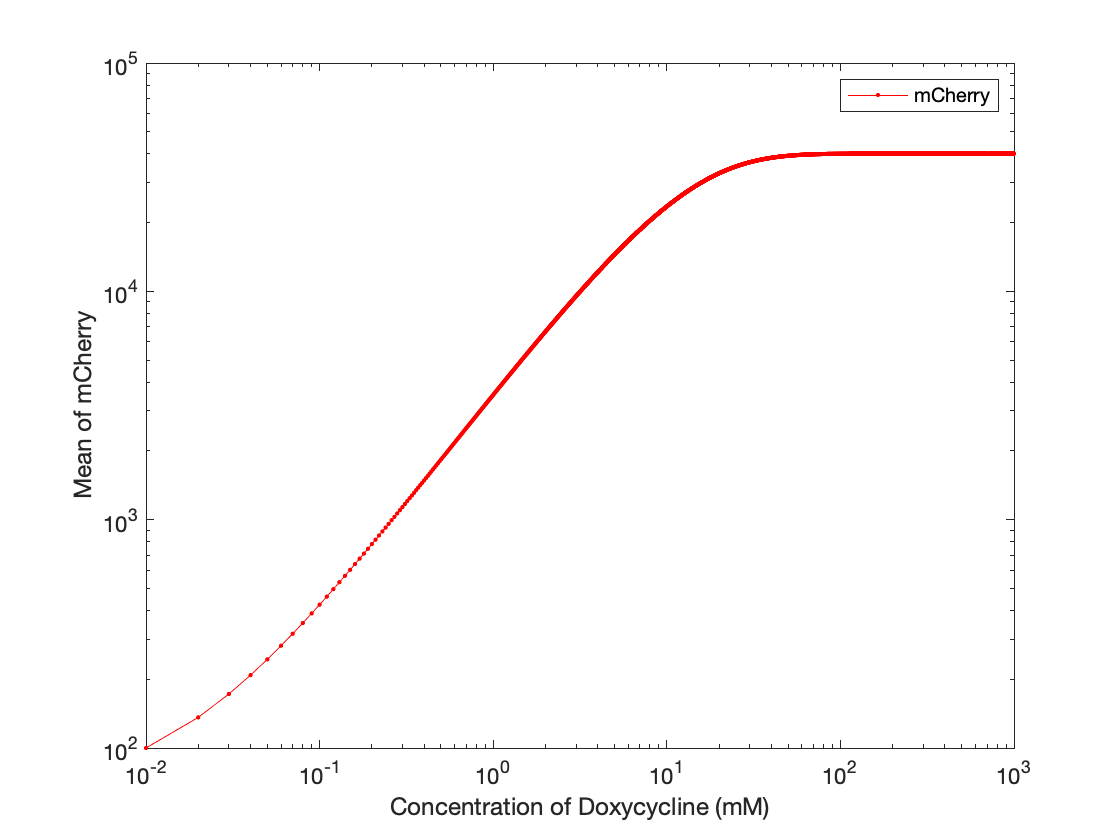
\includegraphics[width=1.0\linewidth]{Figures/Q2_1.png}
\caption{The modeling results for mCherry with feedback}
\label{part_2_model}
\end{figure}

$$K_2 = 1000 mM^{-1}; \sigma_1 = 0.5; K_4 = 0.001 mM^{-1}; \sigma_2 = 0.5;y_0 = 100mM;[R^2_0]_0 = 1000mM$$ 
$$\alpha_1 = 4000 ;\alpha_2 = 4000 ; kdc = 0.01h^{-1} ; kdrd = 0.005h^{-1} ; rc = 10mM*h^{-1} ; rrd = 10mM*h^{-1}$$



%----------------------------------------------------------------------------------------
\newpage
\section{Discuss the differences between Figures \ref{part_2_qestion_figure} F and \ref{part_1_qestion_figure} C, and explain them using the model}

Both the fluorescence of GFP with no feedback and the fluorescence of mCherry with feedback are increased when the concentration of Doxycycline increased. But the processes are quite different.

For the modeling results for GFP with no feedback (shown as Figure 1.2), The slope of curve is changed, it is larger when the Dox concentration is near 1$mM$ while is smaller in two side. Without feedback, the increasing GFP expression does not influencing the system itself. So that there is a threshold for concentration of Dox, when it reaches the threshold, the expression level of the target increases rapidly until the limit is reached.

For the modeling results for mCherry with feedback(shown as Figure 2.2), The slope of the curve is nearly unchanged, so it seems to be a line, which means the expression of mCherry is much more relates to the concentration of Dox. With feedback, the influence of dox is sensed, and the increasing tetR expression inhibits its own expression by binding to the promoter. The expression of the mCherry increases slowly, due to the suppression, and it’s more stable and was directly changed by Dox.



